%%
% This is an Overleaf template for scientific articles and reports
% using the TUM Corporate Desing https://www.tum.de/cd
%
% For further details on how to use the template, take a look at our
% GitLab repository and browse through our test documents
% https://gitlab.lrz.de/latex4ei/tum-templates.
%
% The tumarticle class is based on the KOMA-Script class scrartcl.
% If you need further customization please consult the KOMA-Script guide
% https://ctan.org/pkg/koma-script.
% Additional class options are passed down to the base class.
%
% If you encounter any bugs or undesired behaviour, please raise an issue
% in our GitLab repository
% https://gitlab.lrz.de/latex4ei/tum-templates/issues
% and provide a description and minimal working example of your problem.
%%


\documentclass[
  english,        % define the document language (english, german)
  font=times,     % define main text font (helvet, times, palatino, libertine)
  onecolumn,      % use onecolumn or twocolumn layout
]{tumarticle}


% load additional packages
\usepackage{graphicx}
\graphicspath{./images/}


% article metadata
\title{Eventually Consistent and Resilient CBDC System
}
\subtitle{Introductory talk for the Master’s thesis}
% \author[]{Name: Nadeeshani A W W A \\[-2cm]{ \small Supervisor: A.D.Visor} \\[0cm]{\small Advisor: A.D.Visor}}
% \affil[]{}
\author[]{}
\affil[]{}
\date{}
% \affil[mark=1]{\theDepartmentName, \theUniversityName}

\begin{document}

\maketitle


\vspace{0.5em} \noindent \textcolor{TUMBlue}{ \textbf{Name:}\hspace{3em}} Nadeeshani A. W. W. A \\
\textcolor{TUMBlue}{ \textbf{Supervisor:}\hspace{0.8em}} Prof. Dr.-Ing. Georg Carle \\
\textcolor{TUMBlue}{ \textbf{Advisors:}\hspace{1.6em}} Peter Zeller, Kilian Glas, Filip Rezabek, Richard von Seck \\
{ \noindent \line(1,0){44em}}
\vspace{0.5em}

\section{Introduction}
\hspace{2em}Central Bank Digital Currency (CBDC) is a digital form of a national currency service designed to provide convenient, cost-effective, and secure digital payments.  Availability, Security, Resilience, and Consistency \cite{zhang2022blockchain} are essential properties of such a system to ensure correct and continuous service. The primary objective of this thesis is to explore and develop an enhanced distributed transaction processor protocol that guarantees resilience and low latency.

\section{System Constraints  \& Problem Statement}
\hspace{2em}The CBDC system at G+D is a permissioned distributed network that is scalable from 2 to 10 nodes. The permissioned in the sense that participants on the network can controlled. Moreover, the system already prevents double-spending attempts by both the utilization of an appropriate data representation model and a traditional transaction database layer. Therefore, achieving consensus among the distributed nodes, when some of them may be unreliable or malicious is the main focus of this thesis.

\hspace{1em}In summary, the research problem can be stated as follows: Explore and integrate a tailored consensus protocol that enhances the transaction process in the permissioned distributed CBDC system at G+D, while effectively detecting and mitigating attacks on adversary nodes.

\section{Background \& Motivation}
\hspace{2em} A CBDC system is expected to encounter deliberate malicious nodes that are driven by economic incentives. In the presence of malicious nodes, the distributed system is unable to reach an accurate consensus. This form of failure is commonly described as the Byzantine General's Problem \cite{lamport2019byzantine}. The consensus algorithms are practical solutions designed to address such problems in distributed systems. 

\hspace{1em} A consensus algorithm plays a key role in a CBDC system because it helps to achieve an accurate agreement with the presence of adversary nodes but without any central authority. However, existing CBDC at G+D requires an efficient, faster, and fault-tolerant consensus algorithm that saves computing resources and relies on a smaller group of nodes.

\section{Related Work}
\hspace{2em} Designing and implementing different consensus algorithms has become a popular research topic due to the rapid progress of blockchain and its associated applications. While different algorithms exist, their suitability for a distributed system largely depends on the specific application, bringing both advantages and disadvantages into consideration.

\hspace{1em} The most well-known consensus protocol is Proof of Work (PoW) which is used in Bitcoin \cite{lepore2020survey}. In PoW, a node can propose a new transaction (or block) by solving a puzzle and all other nodes should confirm the transaction's validity. If the majority of nodes agree, consensus is reached. The honest majority is the fundamental assumption of PoW-based systems \cite{lepore2020survey}. When malicious nodes hold more than 50\% of computational power, the safety of the system is compromised. Also, most of the participants only verify the produced blocks but are unable to deny the block content when the malicious nodes have controlled half of the resource \cite{zhang2021hybrid}. Adding more miners decreases the chance for attackers to control 51\% of computational power. This does not align with the current design constraints of the CBDC system at G+D, which requires having fewer nodes. Also, PoW demands a lot of computational power which ensures the decentralization of the network. However, this is not suitable for a CBDC system because of high energy consumption and low transaction throughput \cite{bamakan2020survey}. 

\hspace{1em} Proof-of-stake (PoS) is another consensus algorithm that selects transaction proposer based on their stake. Participants get a reward for voting on the correct block. This verification isn't difficult and participants can misbehave by supporting multiple branches of the network to earn rewards \cite{lepore2020survey}. This will benefit malicious actors and confuse the process of achieving a consensus. Because they incline to create multiple conflicting branches. This is fixed by a penalty system making nodes lose some or all of their stake if they supported multiple branches. Transaction processing in PoS strongly depends on nodes that have the most stake which may lead to centralized behavior \cite{bamakan2020survey}. However, introducing and maintaining a stake could be cumbersome and not align with the requirement of CBDC at G+D. 

\hspace{1em} The success of Proof of Work (PoW) has led to the development of numerous new consensus algorithms such as Proof of Authority (PoA), Proof of Vote (PoV), etc. These “Proof of (X)” consensus models rely on utilizing a scarce resource X, which is a significant challenge for malicious actors to acquire easily. Therefore it enhances the system's safety in a decentralised and permission-less manner.

\hspace{1em} Consensus algorithms play a significant role in determining the performance of the distributed system. Depending on the application and performance criteria, various consensus algorithms may be taken into account.  “Proof of (X)” variants of consensus algorithms are mainly used in permission-less (or public) networks due to their scalability and easiness for many nodes to participate and compete. However, permissioned networks tend to adopt lighter consensus protocols like PBFT, Paxos, and Raft \cite{li2020scalable} to improve the transaction throughput and reduce the computational requirements. 

\hspace{1em} Practical Byzantine Fault Tolerance (PBFT) is a classical consensus mechanism that is widely used in permissioned networks. Liskov et al.\cite{castro1999practical} proposed a PBFT algorithm that effectively addresses the Byzantine failures in asynchronous systems compared to previous Byzantine Fault Tolerance (BFT) algorithms such as Rampart and SecureRing. Byzantine fault tolerance ensures liveness and safety, even in the presence of malicious nodes. PBFT is a consensus protocol designed to operate in partially synchronous systems with 3f+1 nodes when f is the number of Byzantine nodes. A network with n nodes would have to perform 2n\textsuperscript{2} + n number of communications to reach consensus. This is not expected to be a major problem,  as the G+D's CBDC project envisions the participation of just 2 to 10 nodes. However, PBFT doesn't ensure consensus when the total number of nodes is fewer than 4. The above-described classical PBFT has its own drawbacks. However recent research efforts have successfully managed to optimize the classical PBFT consensus algorithm. Reducing the cost of communication, minimizing message delays, and enhancing the performance of read-only operations represent some of the main optimization directions.

\hspace{1em} Certain consensus algorithms designed for permissioned networks offer only Crash Fault Tolerance (CFT) without protection against malicious attacks. These CFT algorithms are a good fit for networks where node trustworthiness is assured. Raft is one example that focuses on crash fault tolerance.

\hspace{1em} The Paxos algorithm \cite{lamport2019part} was introduced in 1990 by Lamport to address the Byzantine General's Problem. In 2013,  Diego Ongaro and John Ousterhout \cite{ongaro2014search} presented the RAFT algorithm as a more convenient alternative to Paxos. RAFT follows a “leader and follower” model, in which a leader node is elected and its decisions are replicated by the followers \cite{hyperledger}. The RAFT consensus protocol can continue to function even if a minority of the servers, such as 2 out of 5 nodes fails. Hyperledger Fabric \cite{hyperledger}, a leading permissioned blockchain, has validated the crash fault tolerance and performance of the RAFT consensus algorithm by effectively incorporating it into its consensus mechanism. Within the RAFT protocol, nodes can be a leader, follower, or a candidate. The leader broadcasts a client’s  transaction to the rest of the nodes. After the non-leader nodes validate and commit this transaction, they send a confirmation response to the leader.  When the leader receives responses from the majority of the nodes, the leader proceeds to commit the transaction and broadcasts this information to all nodes. Finally, consensus is achieved when the follower nodes receive the confirmation of message commitment from the leader 

\hspace{1em} The project Hamilton \cite{lovejoy2023hamilton}  managed to use the Two-Phase Commit (2PC) consensus protocol to achieve high-performance transaction processing. Hamilton's key privacy design involves splitting the transaction process into two main phases, transaction validation and transaction execution. The transaction execution phase (or back-end commit protocol) follows the 2PC design. In 2PC, each transaction is associated with a coordinator. The Coordinator gathers already validated transactions from the validation phase. As the name implies, 2PC consists of two phases; PREPARE and COMMIT. The coordinator sends the transaction to the rest of the nodes (shards) and requests to lock the input. The lock status will be sent back to the coordinator by the nodes. Then the coordinator informs the associated node(s) to complete the transaction. Shards either roll back failed transactions or complete the execution.  

\hspace{1em} Hamilton’s Unspent funds Hash Set (UHS) ormain database is partitioned across multiple shards for scalability of both the database size and the throughput. It uses 2PC for coordination between partitions in combination with conservative two-phase locking (C2PL). C2PL protects the UHS from conflicting transactions. Moreover, coordinators and shards are RAFT-replicated for fault tolerance and high availability.

\section{Objectives \& Work Plan}
\hspace{2em} The primary intention of this thesis is to integrate a suitable transaction-processing protocol into the CBDC network at G+D that operates with a limited number of nodes. However, finding an optimal solution depends on the current system's characteristics, such as data model representation, security properties, etc. The solution should effectively address transaction processing speed, throughput, scalability, and resiliency. The objectives of this thesis can summarized as follows. 
\begin{enumerate}
\item Research on a suitable improved transaction protocol that guarantees the liveness and safety of the existing CBDC system at G+D.
\item Implementing a prototype based on the findings and integrating it into the existing system.
\item Finding proper benchmarks and evaluating the performance of the newly developed system.
\item Evaluate the results and optimize the final solution.
\end{enumerate}
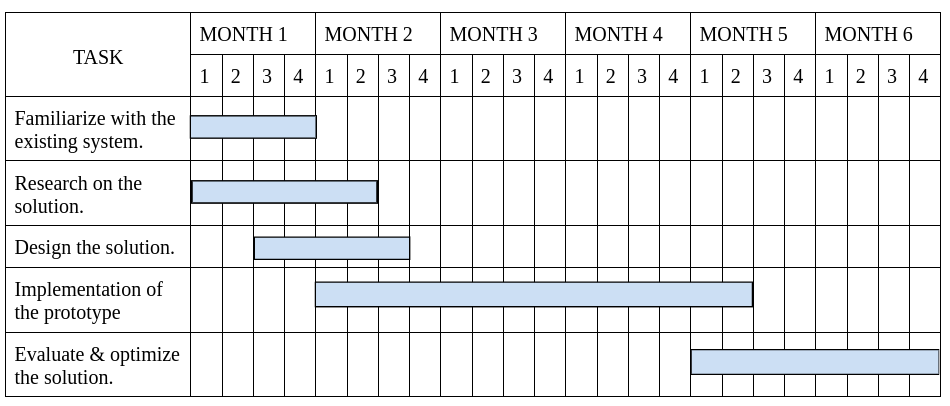
\includegraphics[scale=0.5]{images/timeline.png}

\bibliographystyle{ieeetr}
\bibliography{references}

\end{document}
